% Requires preamble: \usepackage{amsthm,amsmath,amssymb}
% and: \newtheorem{theorem}{Theorem}
%      \newtheorem{corollary}[theorem]{Corollary}
%      \newtheorem{proposition}[theorem]{Proposition}

\section{Bias Decomposition: When Debiasing Hurts}
\label{sec:theory}

We formalize the bias that global misclassification correction introduces when subgroup error rates are heterogeneous.
Consider estimating the conditional average treatment effect (CATE) $\tau(z) = \mathbb{E}[Y(1) - Y(0) \mid Z = z]$, where $Z \in \{0, 1\}$ is a binary effect modifier observed only through a noisy annotation $\hat{Z}$.
The population consists of $K$ subgroups $S \in \{1, \ldots, K\}$ with weights $w_s = P(S{=}s)$, each characterized by a $2 \times 2$ confusion matrix $C_s$ with symmetric error rate $\pi_s = P(\hat{Z} \neq Z \mid S{=}s)$.
Standard practice estimates a single confusion matrix $\bar{C} = \sum_s w_s C_s$ from expert annotations and applies its inverse uniformly to all observations, with pooled error rate $\bar{\pi} = \sum_s w_s \pi_s$.
We show that when error rates vary across subgroups, this global procedure introduces a bias with an exact product form.

We state five assumptions maintained throughout.
%
\begin{itemize}
\item[\textbf{(A1)}] \textit{Conditional independence:} misclassification depends only on the true label $Z$ and subgroup $S$, not on potential outcomes $Y(0), Y(1)$.
\item[\textbf{(A2)}] \textit{Symmetric misclassification (expository simplification):} $P(\hat{Z}{=}1 \mid Z{=}0, S{=}s) = P(\hat{Z}{=}0 \mid Z{=}1, S{=}s) = \pi_s$ for all $s$. Used only to reduce $[B_s]_{z,1}$ to the scalar $\pm\delta_s/(1{-}2\bar{\pi})$; the product-form identity holds for arbitrary asymmetric matrices without~(A2) (Remark~\ref{rem:asymmetric}).
\item[\textbf{(A3)}] \textit{Balanced effect modifier:} $P(Z{=}0) = P(Z{=}1) = 0.5$. This simplifies the exposition; we discuss relaxation below.
\item[\textbf{(A4)}] \textit{Better-than-random classifier:} $\pi_s < 0.5$ for all $s$, ensuring each $C_s$ is invertible.
\item[\textbf{(A5)}] \textit{Homogeneous treatment effects across subgroups:} $\tau(z, s) = \tau(z)$ for all $s$, so $\Delta\tau = \tau(1) - \tau(0)$ is a scalar (relaxed to subgroup-specific $\Delta\tau_s$ in Proposition~\ref{prop:a5_relaxation}).
\end{itemize}

Under (A2)--(A3), the Bayesian mixing matrix $M_s$ (entries $M_s[\hat{z}, z] = P(Z{=}z \mid \hat{Z}{=}\hat{z}, S{=}s)$) coincides with $C_s$.
The global mixing matrix is $M_{\text{global}} = \sum_s w_s M_s$.

\begin{theorem}[Bias Decomposition Identity]
\label{thm:bias_identity}
Under \textnormal{(A1)--(A5)}, the bias of global correction in subgroup $s$ at effect-modifier level $z$ is
\begin{align}
\mathrm{bias}_{\mathrm{global}}(z{=}0, s) &= +\frac{\delta_s \cdot \Delta\tau}{1 - 2\bar{\pi}}, \label{eq:bias_z0} \\
\mathrm{bias}_{\mathrm{global}}(z{=}1, s) &= -\frac{\delta_s \cdot \Delta\tau}{1 - 2\bar{\pi}}, \label{eq:bias_z1}
\end{align}
where $\delta_s = \pi_s - \bar{\pi}$ is the subgroup deviation from the pooled error rate and $\Delta\tau = \tau(1) - \tau(0)$ is the CATE heterogeneity.
\end{theorem}

Bias vanishes when either $\delta_s = 0$ (homogeneous errors) or $\Delta\tau = 0$ (no effect heterogeneity), and arises only through their interaction; $1/(1 - 2\bar{\pi})$ amplifies via matrix inversion.
The identity is correction-layer: it characterizes bias introduced by the correction step itself, trading attenuation from label noise for a new bias from error-rate heterogeneity. Propagation to downstream estimators is verified empirically (Section~\ref{sec:bias_mechanism}).

\paragraph{Numerical example ($K{=}2$).}
Suppose two subgroups with $\pi_A = 0.05$, $\pi_B = 0.25$, giving $\bar{\pi} = 0.15$, and true CATEs $\tau(0) = 0.10$, $\tau(1) = 0.30$, so $\Delta\tau = 0.20$.
For subgroup $A$: $\delta_A = -0.10$, bias $= -0.10 \times 0.20 / 0.70 = -0.029$; global correction \emph{creates} bias in a subgroup where the naive estimator is nearly unbiased ($\pi_A = 0.05$).
For subgroup $B$: $\delta_B = +0.10$, bias $= +0.029$, partially offsetting attenuation. The opposite signs illustrate why aggregate metrics can mask subgroup-level harm.

\paragraph{Proof sketch.}
Global correction applies $M_{\text{global}}^{-1}$ to the subgroup-specific observed CATE $\tau_{\text{obs}}(\cdot, s) = M_s \cdot \tau_{\text{true}}$, yielding bias $(M_{\text{global}}^{-1} M_s - I) \cdot \tau_{\text{true}}$.
Direct computation shows $M_{\text{global}}^{-1} M_s - I = \frac{\delta_s}{1-2\bar{\pi}} \bigl[\begin{smallmatrix} -1 & 1 \\ 1 & -1 \end{smallmatrix}\bigr]$.
Applying this matrix to $[\tau(0),\, \tau(1)]^\top$ produces the product form.
The full derivation appears in Appendix~\ref{app:derivation}.
Unlike Frazis--Loewenstein (F-L) scalar attenuation~\citep{frazis2003estimating}, which uniformly shrinks estimates toward zero ($K{=}1$: $\delta_s \equiv 0$ recovers $\hat{\beta} = (1-2\pi)\beta$), the product form reveals that correction can \emph{reverse} bias sign across subgroups, a qualitatively new phenomenon from error-rate heterogeneity invisible to any global-scalar analysis (F-L increases $|\text{bias}|$ to $0.122$, $2.1\times$ naive; Table~\ref{tab:main_results}).

\begin{remark}
\label{rem:asymmetric}
Theorem~\ref{thm:bias_identity} does not require~(A2).
For arbitrary asymmetric confusion matrices (CMs), the product form $\mathrm{bias}(z, s) = \Delta\tau \cdot [B_s]_{z,1}$ holds exactly with $B_s = M_{\mathrm{global}}^{-1} M_s - I$, since $B_s \mathbf{1} = \mathbf{0}$ follows from stochasticity alone; (A2) only simplifies $[B_s]_{z,1}$ to the scalar $\pm \delta_s / (1{-}2\bar{\pi})$.
Under asymmetric errors, the diagnostic (Proposition~\ref{prop:debiasing_hurts}) with $\pi_s = (\mathrm{FPR}_s + \mathrm{FNR}_s)/2$ (where FPR and FNR denote false positive and false negative rates) achieves area under the ROC curve (AUC) $= 0.96$ across 48 configurations and correctly identifies all harmed subgroups across 8 semi-real LLM CMs (Appendix~\ref{app:asymmetric}).
\end{remark}

\begin{proposition}[Exact Identity under Heterogeneous Treatment Effects]
\label{prop:a5_relaxation}
When $\tau(z, s)$ varies across subgroups (relaxing A5), the bias identity remains exact:
\begin{align}
\mathrm{bias}_{\mathrm{global}}(z{=}0, s) &= +\frac{\delta_s \cdot \Delta\tau_s}{1 - 2\bar{\pi}}, \label{eq:hetero_z0} \\
\mathrm{bias}_{\mathrm{global}}(z{=}1, s) &= -\frac{\delta_s \cdot \Delta\tau_s}{1 - 2\bar{\pi}}, \label{eq:hetero_z1}
\end{align}
where $\Delta\tau_s = \tau_s(1) - \tau_s(0)$ is the subgroup-specific CATE heterogeneity.
\end{proposition}

\begin{corollary}[Aggregate Bias]
\label{cor:aggregate_bias}
The population-weighted aggregate bias is $\mathrm{Cov}_w(\pi_s, \Delta\tau_s) / (1 - 2\bar{\pi})$.
\end{corollary}

The proof is immediate: $B_s$ depends only on confusion matrices, so the diagnostic extends unchanged and EC-HTE maintains $\geq$93\% coverage under both correlation signs (Appendix~\ref{app:a5_violation}).

\begin{figure}[t]
\centering
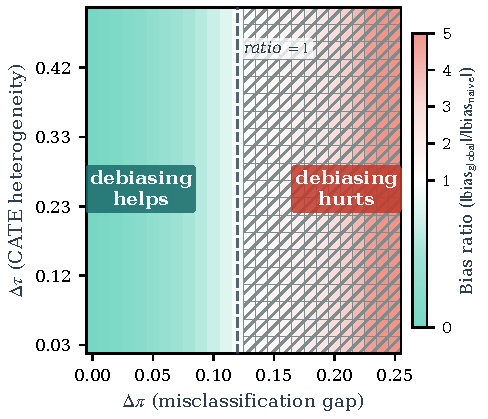
\includegraphics[width=\columnwidth]{figures/fig2_heatmap.pdf}
\caption{Bias amplification under global correction ($K{=}2$, low-error subgroup $\pi_s < \bar{\pi}$). Correction \emph{increases} bias when $\Delta\pi > 0.12$ (hatched), reaching $2.86\times$. High-error subgroups ($\pi_s > \bar{\pi}$) always have ratio $< 1$ (correction helps); see Appendix~\ref{app:dgp}.}
\label{fig:heatmap}
\end{figure}

The identity extends to $K > 2$ with $J$ effect-modifier levels (Corollary~\ref{cor:multiclass}, Appendix~\ref{app:multiclass}).
Under class imbalance (relaxing A3), the identity remains exact ($R^2 \geq 0.976$ at $P(Z{=}1) = 0.1$), though EC-HTE's RMSE advantage narrows (Appendix~\ref{app:classimbalance}).
Empirical verification yields $R^2 = 0.994$ ($K{=}2$) and $0.97$ ($K{=}4$; Section~\ref{sec:bias_mechanism}).
If (A1) is violated (treatment-dependent misclassification strength $\gamma_T = 0.10$), coverage degrades to 75\% (Appendix~\ref{app:treatment_dep}).
The finite-sample remainder is $R_n = O_p(n_{\text{expert}}^{-1/2} \cdot \kappa(C_s)^2)$, motivating the $\kappa$-guard in Section~\ref{sec:method}.

\begin{proposition}[Debiasing Can Increase Bias]
\label{prop:debiasing_hurts}
Under \textnormal{(A1)--(A5)}, global correction produces larger absolute bias than the naive estimator ($|\mathrm{bias}_{\mathrm{global}}| > |\mathrm{bias}_{\mathrm{naive}}|$) in subgroup $s$ if and only if
\begin{equation}
\frac{|\delta_s|}{(1 - 2\bar{\pi}) \cdot \pi_s} > 1.
\label{eq:hurts_condition}
\end{equation}
\end{proposition}

Equation~\eqref{eq:hurts_condition} partitions subgroups into two regimes.
For high-error subgroups ($\pi_s > \bar{\pi}$), the condition reduces to $\pi_s > 0.5$, excluded by~(A4); global correction always reduces bias.
For low-error subgroups ($\pi_s < \bar{\pi}$), the condition holds whenever $\pi_s < \bar{\pi} / (2(1{-}\bar{\pi}))$, which is easily satisfied: when $\bar{\pi} = 0.15$, any subgroup with $\pi_s < 0.088$ is harmed by global correction.
The mechanism is over-correction: for subgroups with near-zero misclassification, the naive estimator is nearly unbiased, yet global inversion calibrated for $\bar{\pi}$ creates substantial bias (proof in Appendix~\ref{app:debiasing_hurts}).
In our experiments, global correction increases bias in 50\% of $K{=}2$ configurations (260/520), with amplification reaching $2.86\times$ ($K{=}2$) and $2.41\times$ ($K{=}4$); Figure~\ref{fig:heatmap} visualizes the full parameter grid.